%************************************************
\chapter{Introduction}\label{ch:introduction}
%************************************************
\section{Background and Context}
Autonomous systems are complex agents capable of carrying out operations without human intervention. They have become more capable thanks to technological advancements and increasingly integrated into society with recent remarkable progress in artificial intelligence (AI) techniques. According to Zhang in \cite{Zhang2017}, current trends indicate that the development and adoption of such systems will continue to grow in the coming years.  

The agricultural sector is one of the areas where the integration of autonomous technologies has great potential. These systems could significantly benefit farmers by making their work safer and less repetitive. Autonomous systems have already been used in alternative cropping methods such as precision agriculture. Nevertheless, traditional practices are still facing challenges that autonomous systems could perfectly address. Among these challenges, the proliferation of weeds in grass fields raises as a major concern for the livestock well-being for two main reasons. First, weeds compete with grass for resources, reducing the quality of food available for grazing animals. Second, some weed species pose a direct threat to livestock health. In particular, plants like Rumex have been identified as toxic and the cause of livestock poisoning \cite{Panciera1990}.

Removing these plants is a task that farmers must perform manually, as EU regulations restrict the use of pesticides and prevent farmers from combating weed proliferation through chemical means. It is evident that this task, especially in large grass fields, is highly time-consuming and extremely repetitive, making it an ideal candidate for automation. In Germany, companies like Paltech have developed solutions to address this problem using autonomous wheeled robots. Their flagship robot is a differential-drive wheeled system equipped with various sensors for localization and weed detection, as well as an onboard drilling mechanism for weed removal. Currently, if the weed removal process needs to be sped up, the only solution is to deploy a fleet of robots. While this is feasible, developing single units capable of holding more than one drilling mechanism seems like the natural next step in Paltech's solution.

\section{Problem Statement}
% 1) What is the problem, why is it important? \\

The development of systems with more than one drilling unit for weed removal comes with both hardware and software challenges. It is crucial to ensure that tools and system resources are used as efficiently as possible. We want to avoid having more capable units with unused tools, especially since the production and deployment of these improved systems are more costly. Therefore, reducing idle time is a top priority and the focus of this thesis.

% 2) What are the technology challenges, and, in particular, what are the overall areas that must be addressed to solve the technical aspects of the problem? \\

Idle time refers to periods when resources, such as drilling equipment, are not actively engaged in productive work. Reducing idle time in this context means minimizing the time tools remain unused and maximizing their productivity in weed removal. To achieve this, allocating detected plants to the correct tools is essential. In the literature, this process is known as task allocation. Some technical challenges to consider during implementation include computational latency and multi-tool coordination. The task allocation algorithm and execution pipeline must be fast enough to process new detections and reassign tools in real time without causing delays, while also ensuring that multiple drilling units operate efficiently without interference or redundancy.

\section{Current Solutions}
% 3) What are the capabilities of the current technology in the literature? \\

In general, a task allocation system aims to achieve an efficient assignment of tasks to robots (or tools in this case) by considering various characteristics such as the robots' capabilities, task requirements, and system efficiency. This process of task allocation involves three important factors to be consider acording to Umashankar in \cite{10.1145/3700591}. Robot/tool, environment and coordination as shown in Figure \ref{fig:task-allocation-classification}. 

\begin{figure}[bth]
    \centering
    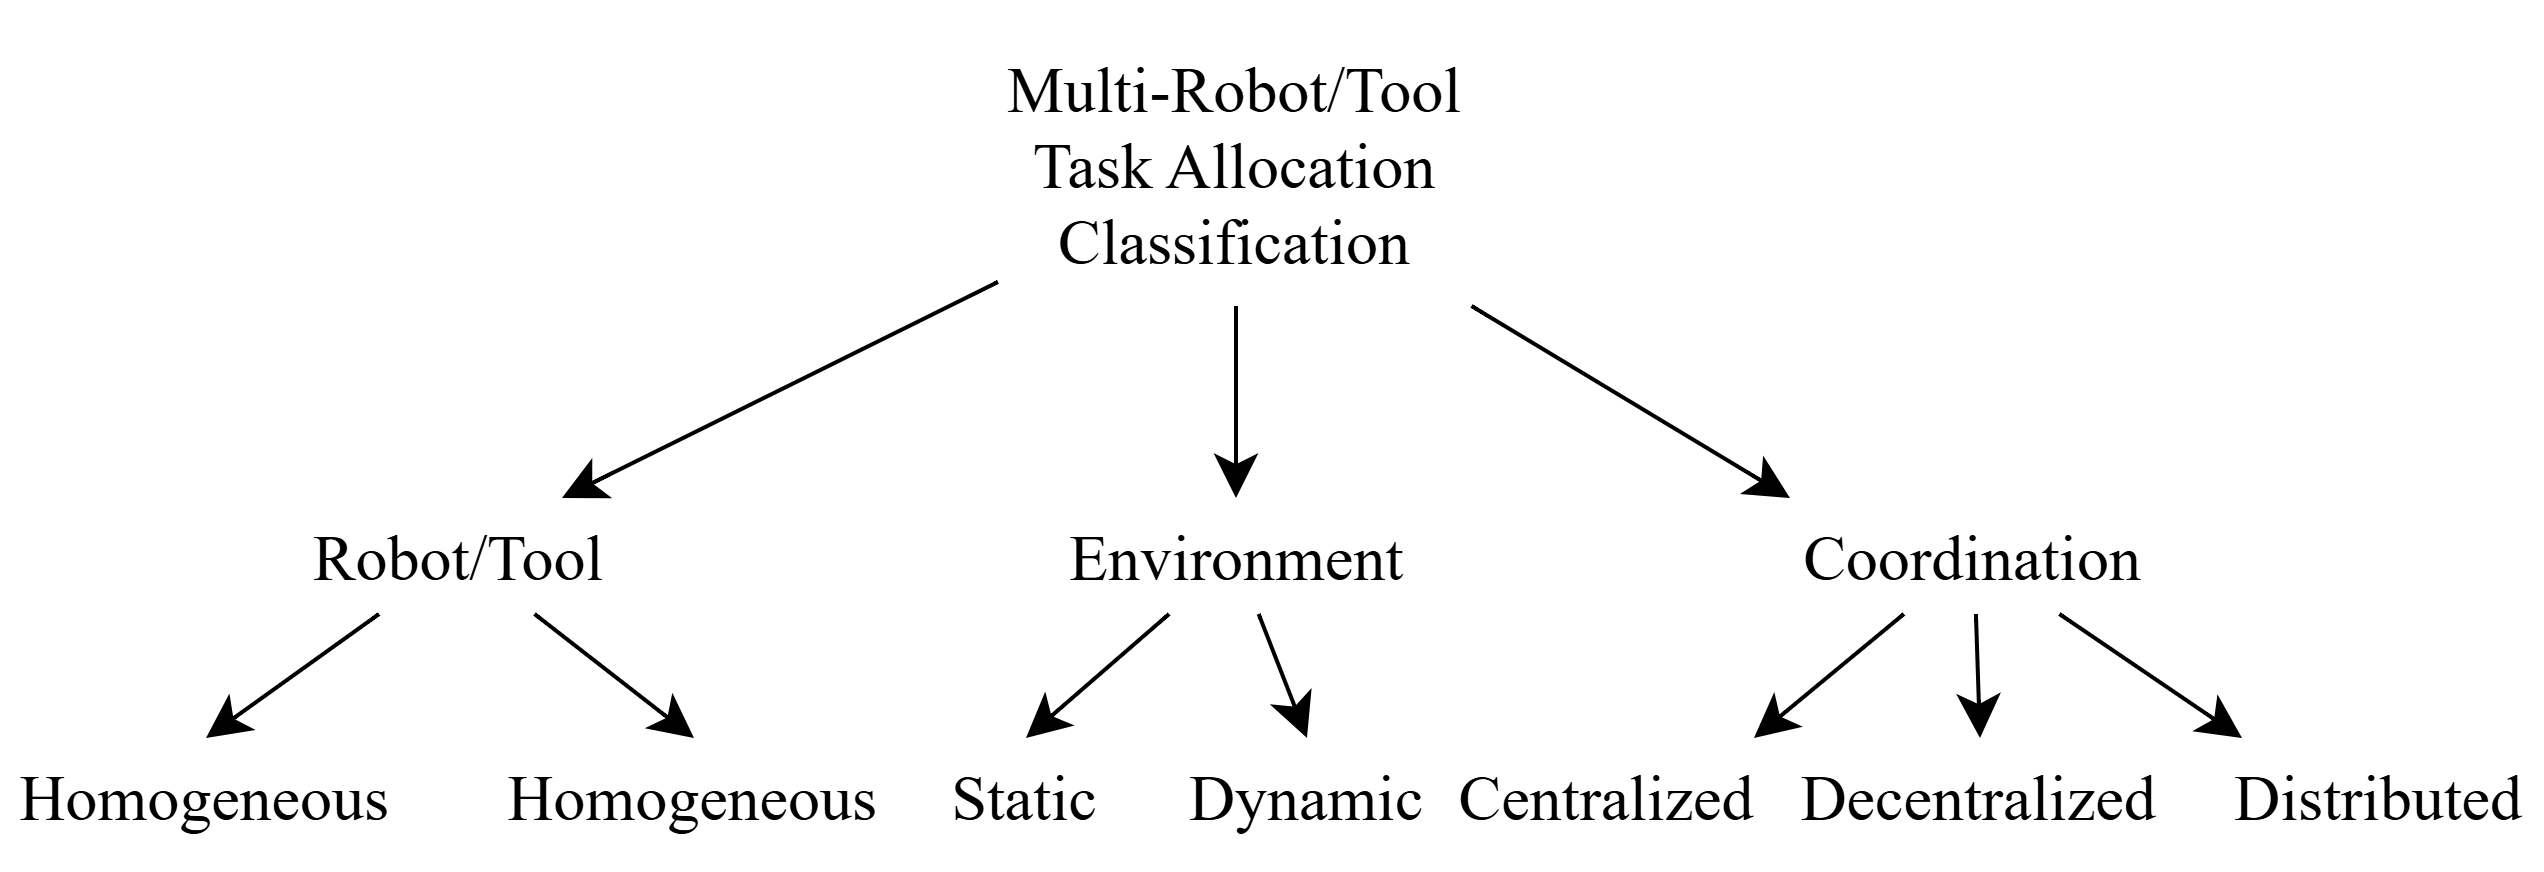
\includegraphics[width=0.9\linewidth]{gfx/ch01/task-allocation-classification.png}
    \caption{Multi-robot/tool task allocation classification. Source \cite{10.1145/3700591}}
    \label{fig:task-allocation-classification}
\end{figure}

An example of homogeneous tools in this context is a robot equipped with multiple tools of the same type, such as drills. In contrast, heterogeneous tools refer to robots equipped with different types of tools, such as drilling, seeding, and sensing equipment.

The multi-tool task allocation can take place in either a dynamic or static environment. In an environment that is static in nature, tasks are allocated to tools in advance before they begin to execute them. This method works well in situations when the tasks are predetermined and the environment remains unchanged. In contrast, dynamic task allocation involves the real-time assignment of tasks to tools as they carry out their activities. For the scope of this thesis, we will focus on homogeneous tools operating in a dynamic environment with centralized coordination, where the onboard computer will act as the master, assigning plants to each drilling mechanism.

There are several ways to accomplish multi-tool allocation, including heuristic, cluster-based, market-based, learning-based, and optimization-based techniques. Table \ref{tab:task-allocation-approaches-1} and \ref{tab:task-allocation-approaches-2} presents a comprehensive classification of task allocation algorithms found in the literature.

\begin{table}[bth]
    \centering
    \renewcommand{\arraystretch}{1.2} % Adjust row height
    \begin{tabular}{|l|l|}
        \hline
        \textbf{Approach} & \textbf{Technique/Algorithm} \\ 
        \hline
        \multirow{7}{*}{Cluster Based} & SVCA \cite{MARTIN2023104314} \\ 
        & Group Agent Partitioning \cite{9423979} \\ 
        & Consensus-Based Distributed Task Allocation \cite{8584210} \\ 
        & Voronoi Diagram-Based, K-Means Algorithm \cite{8970316}\\ 
        & CBBA \cite{6787310} \\ 
        & Cluster First Consensus-Based Strategy \\ 
        & K-Means Clustering \\ 
        \hline
        \multirow{16}{*}{Market Based} & Auction Algorithm \cite{10023897} \\
        & Improved Auction Algorithm \cite{9501305} \\
        & Extended auction algorithm \\
        & Distributed auction algorithm \\
        & Sequential single-item auctions \\
        & Auction-based algorithm \\
        & Multihop-based auction algorithm \\
        & Based on sequential single item auctions \\
        & Consensus Based Parallel Auction and Execution Algorithm \\
        & Extended sequential single item auction \\
        & Distributed auction-based algorithm \\
        & The consensus-based bundle algorithm \\
        & Linear integer programming \\
        & Contract Net protocol \\
        \hline
    \end{tabular}
    \caption{Different Approaches to Task Allocation, Source \cite{10.1145/3700591}}
    \label{tab:task-allocation-approaches-1}
\end{table}

\begin{table}[H]
    \centering
    \renewcommand{\arraystretch}{1.2} % Adjust row height
    \begin{tabular}{|l|l|}
        \hline
        \textbf{Approach} & \textbf{Technique/Algorithm} \\ 
        \hline
        \multirow{9}{*}{Learning Based} 
        & Gated Recurrent Unit, Multi-layer Perceptron \cite{9700783} \\
        & Deep Reinforcement Learning \cite{app11072895} \\
        & Heterogeneous Graph Attention Network \\
        & Capsule Attention-based Mechanism \\
        & Encoder Decoder Architecture with cross attention mechanism \\
        & Graph Neural Network (GNN) \\
        & Q-Learning , Convolutional layers and a GRU \\
        & Deep Reinforcement Learning \\
        & Graph Convolutional Neural Networks \\
        \hline
        \multirow{15}{*}{Optimization Based} 
        & Mixed-integer quadratic program \\
        & Centralized Hungarian method \cite{Lindsay2021} \\
        & Bin Maximum Item Doubled Packing \\
        & Particle swarm optimization (PSO) algorithm \\
        & Group theory and Optimization duality theory \\
        & Particle Swarm Optimization \\
        & Group theory and the optimization duality theory \\
        & Integer Programming \\
        & Mixed-integer quadratic program (MIQP) \\
        & A genetic algorithm (GA), A* algorithm \\
        & Constraint based optimization as quadratic program \\
        & Particle Swarm Optimization \\
        & Heuristic based \\
        & Diferential Evolution for multimodal problems \\
        & Fuzzy Optimization \\
        \hline
    \end{tabular}
    \caption{Different Approaches to Task Allocation, Source \cite{10.1145/3700591}}
    \label{tab:task-allocation-approaches-2}
\end{table}

In cluster-based approaches, the goal is to group tasks into a predefined number of clusters. Instead of assigning a single task to each tool, the clustering approach allocates entire groups of tasks to them, reducing the number of individual task assignments and computational complexity. Clustering approaches aim to minimize travel distance and maximize task coverage by grouping tasks effectively. However, the optimal clustering of tasks still needs further exploration. Although these approaches simplify task allocation, they struggle to handle dynamic changes in the environment.

An optimization-based strategy aims to select the best solution from a set of available options. These solutions are constrained by specific conditions, and the optimal one is determined based on the objective function. The objective function represents the system's ultimate goal. Some of the optimization algorithms have poor robustness to uncertainties therefore this approach is more suitable for solving well-defined and static problems focusing on theoretically optimal or near-optimal solutions. Additionally, optimization-based approaches require more computational power and are less adaptable to changing environments.

Market-based approaches effectively handle highly combinatorial optimization problems. In this method, an auctioneer informs agents about available tasks and requests bids. Each agent evaluates its capacity to complete the tasks and submits a bid accordingly. The auctioneer then assigns tasks to the agent with the most favorable bid. Generally, task allocation using this approach minimizes travel time. While these methods are flexible and scalable, they may not always achieve a globally optimal solution.

Recent approaches to task allocation incorporate deep learning techniques such as graph neural networks and graph convolutional networks. These types of task allocation methods are commonly referred as learning-based approaches. Most learning-based approaches struggle to generalize to larger-scale problem scenarios beyond those used during training. This characteristic is especially important because real-world task allocation problems frequently require modeling scenarios whose costs increase with the number of tasks and robots. Table \ref{tab:approaches-comparison} gives a comparison between all the approaches.

% 4) What are the technical gaps that remain? \\

\begin{table}[H]
    \centering
    \renewcommand{\arraystretch}{1.3} % row height
    \makebox[\textwidth]{
    \begin{tabular}{|p{2.0cm}|p{2.5cm}|p{3.0cm}|p{2.5cm}|p{2.5cm}|}
        \hline
        \textbf{} & \textbf{Clustering} & \textbf{Optimization} & \textbf{Market-Based} & \textbf{Learning-Based} \\ 
        \hline
        \textbf{Advantage} & Simplifies task allocation and reduces complexity & Provides optimal solutions, well suited for static problems & Flexible, scalable, decentralized & Adaptable, learns, and improves over time \\
        \hline
        \textbf{Limitation} & May not account for dynamics well & Computationally intensive, less adaptable & May not yield global optima, and needs effective bidding & Requires training time, initially sub-optimal \\ 
        \hline
        \textbf{Best case} & Logical tasks & Well-defined, static problems & Dynamic environments with varying tasks & Complex and uncertain environments \\ 
        \hline
        \textbf{Future work} & Dynamic clustering, online adaptation & Hybrid models, real-time optimization & Adaptive market mechanisms, incentive models & Transfer learning, meta-learning \\
        \hline
    \end{tabular}
    }
    \caption{A Comparison of different approaches to TA, Source \cite{10.1145/3700591}}
    \label{tab:approaches-comparison}
\end{table}

\section{Proposed Solution}
% 5) What are the proposed solution approaches?
As Table \ref{tab:approaches-comparison} illustrates, algorithm selection must be carefully considered based on the application's nature to achieve optimal performance. In a grass field clearing application, the environment is highly dynamic, especially since weed detections occur while the system is in motion. Therefore, market-based approaches are well-suited to ensuring the system adapts effectively to such conditions. However, since weeds often spread in clustered areas, a cluster-based approach could help reduce the algorithm's computational load and improve real-time responsiveness.

A hybrid algorithm is proposed to tackle the dynamics of the environment and leverage the benefits of both market-based and cluster-based approaches. By combining real-time adaptability with efficient task grouping, the system can dynamically allocate tasks while minimizing computational overhead. This approach ensures that weed removal remains efficient even as new detections occur, ultimately improving performance in large-scale and rapidly changing field conditions.